\section{Project Management Review}
\subsection{Current progress}

During the initial stages of the project, time, as denoted in the original time plan, was dedicated to researching the appropriate language to use, the file format and the methods and algorithms used by other packages. This involved looking at the projects done in music in Python previously, such as Music21 \parencite{Music21}, and other projects listed on the Python Foundation website\parencite{pmus}. 

Many important decisions were made from this research period, such as the decision to use Lilypond to typeset music files rather than create a new algorithm and the research of MusicOCR options available, leading to the decision that MusicOCR is too big a topic for this project to create a new algorithm.


After this research period, class diagrams were drawn and some initial code implementation for the rendering and metadata objectives was developed. It was decided after this intial stage to use Test Driven Development, as the code base and algorithm for loading in a music file was becoming hard to confirm crucial details were being parsed correctly. A set of unit tests were written for the initial implementation, and from this point onward the methodology was applied.

\begin{figure}[h]
    \centering
    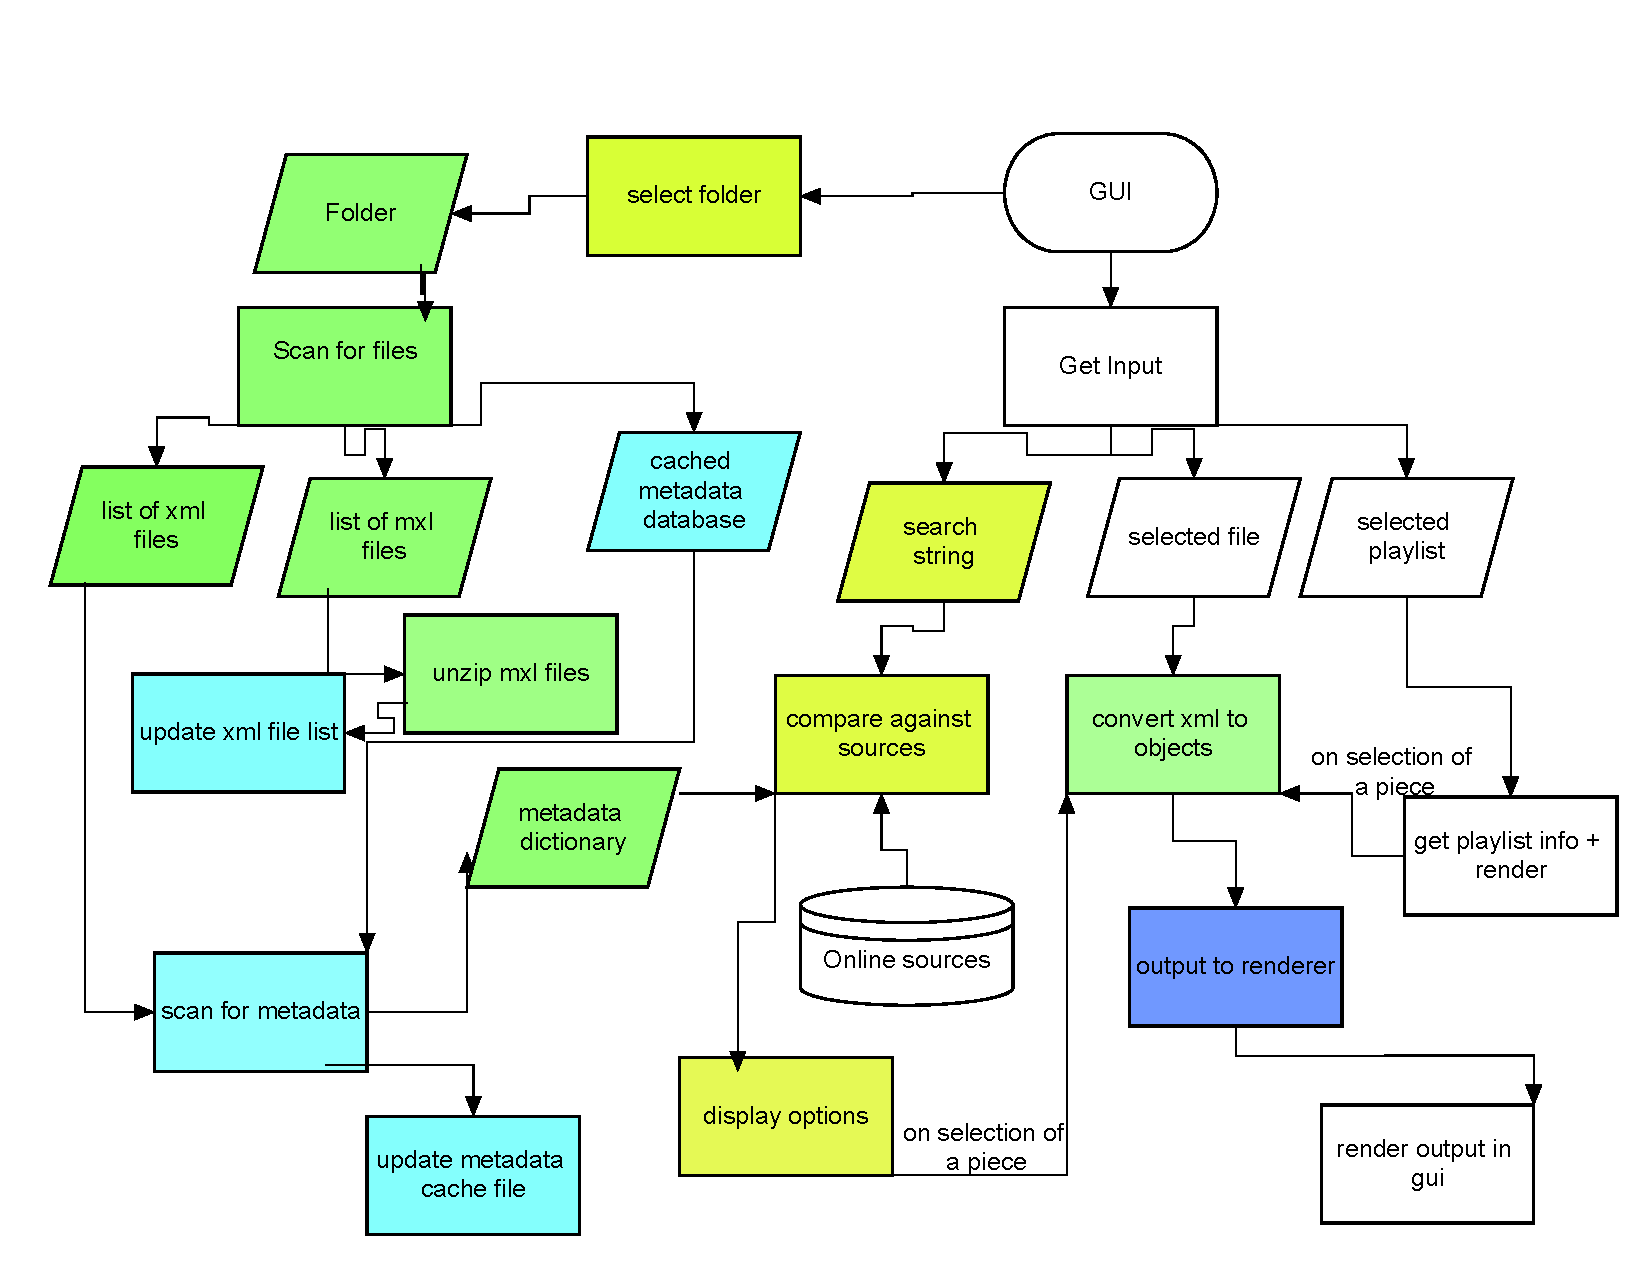
\includegraphics[width=400pt]{flowchart-progress}
    \caption{Flowchart colour coded according to progress}
    \label{colours}
\end{figure}
Figure \ref{colours} shows the flowchart shown in figure \ref{fig:flow} colour coded to show progress. Green indicates that this area is considered complete, light blue indicates that this area has been completed but requires refactoring, yellow indicates that this area has been implemented on a command-line level but requires connection to a user interface to be considered completed, and dark blue indicates the area currently in development.

Of the areas shaded in light blue, the cached metadata database is currently stored as a serialised python object. In order to make this as extendible and portable as possible, this will need to be refactored to using an SQLite file to be considered completed. SQLite is a light implementation of an SQL database stored as a single file, which should be relatively simple to implement in other languages as it is standardised.
\subsection{Adjustments made}
based on coursework deadlines
issues with stress/multiple projects being handled
review and modifications made, and future things to consider in project management based on these

\subsection{Revised timeplan}
decision on objective implementation: OCR